\documentclass[12pt,a4paper,oneside,titlepage]{article}

\usepackage{fontspec}
\setmainfont{DejaVu Serif}
\setsansfont{DejaVu Sans}
\setmonofont{DejaVu Sans Mono}
\defaultfontfeatures{Ligatures=TeX}
\usepackage{polyglossia}
\usepackage[autostyle=true]{csquotes}
\setdefaultlanguage{russian}
\setotherlanguage{english}

\usepackage{listings}
\usepackage{graphicx}
\graphicspath{ {./} }

\lstset{
  columns=fullflexible,
  frame=single,
  breaklines=true,
}

\begin{document}

% НАЧАЛО ТИТУЛЬНОГО ЛИСТА
\begin{center}
  \hfill \break
  \textbf{
    \footnotesize{Министерство науки и высшего образования Российской Федерации}\\
    \hfill \break
    \footnotesize{Федеральное государственное бюджетное образовательное учреждение высшего образования}\\
    \small{«МОСКОВСКИЙ ГОСУДАРСТВЕННЫЙ ТЕХНИЧЕСКИЙ УНИВЕРСИТЕТ имени Н.Э.БАУМАНА\\(национальный исследовательский университет)»}}\\
\end{center}
\hfill \break
\normalsize{Факультет: Информатика и системы управления}\\
\hfill \break
\normalsize{Кафедра: Теоретическая информатика и компьютерные технологии}\\
\hfill\break
\begin{center}
  \textbf{\large{Лабораторная работа №1}}\\
  \large{Базовые средства разработки для языка Java\\
    по дисциплине «Языки и методы программирования»}\\
\end{center}
\hfill \break
\hfill \break
\hfill \break
\begin{flushright}
  \normalsize{
    Выполнил\\
    студент группы ИУ9-21Б\\
    Старовойтов А.И.\\
  }
  \normalsize{
    Проверил\\
    Посевин Д.П.
  }
\end{flushright}
\hfill \break
\hfill \break
\hfill \break
\hfill \break
\hfill \break
\hfill \break
\hfill \break
\hfill \break

\begin{center} Москва, 2022 \end{center}
\thispagestyle{empty} % выключаем отображение номера для этой страницы
% КОНЕЦ ТИТУЛЬНОГО ЛИСТА

\author{Старовойтов Александр}

\section{Цель работы}

формирование комфортного окружения для
разработки ПО на языке Java.

\section{Условия задачи}

\begin{itemize}
  \item
        Установка jdk на ваш компьютер
  \item
        Проверка работоспособности jdk
  \item
        Установка IntelliJ IDEA на ваш компьютер
\end{itemize}

\section{Factorial}

\begin{lstlisting}[language=java]
import java.util.stream.IntStream ;

public class Factorial {
    public static void main (String[] args) {
        if (args.length == 0) {
            System.out.println("usage: java Factorial x");
        } else {
            int n = Integer.parseInt(args[0]);
            int f = IntStream.range(1 , n + 1).reduce(1 , (r , x)->r*x) ;
            System.out.println(f);
        }
    }
}
\end{lstlisting}

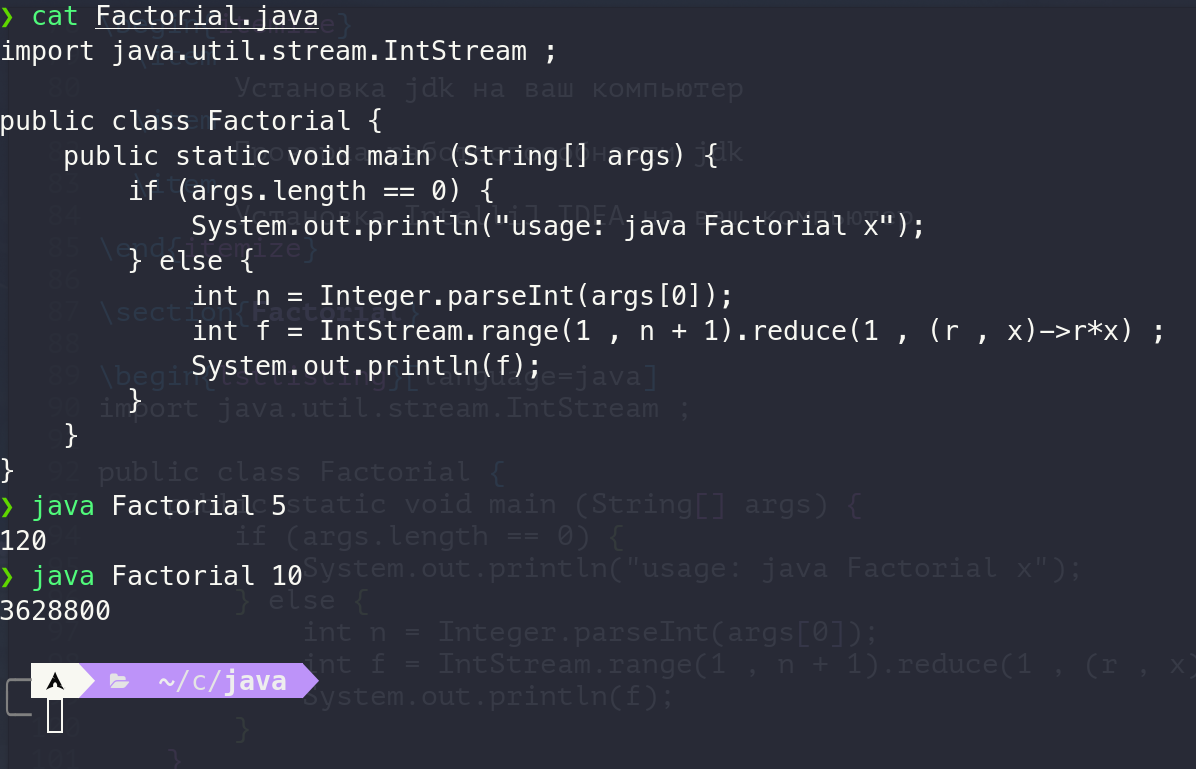
\includegraphics[width=\textwidth]{terminal}
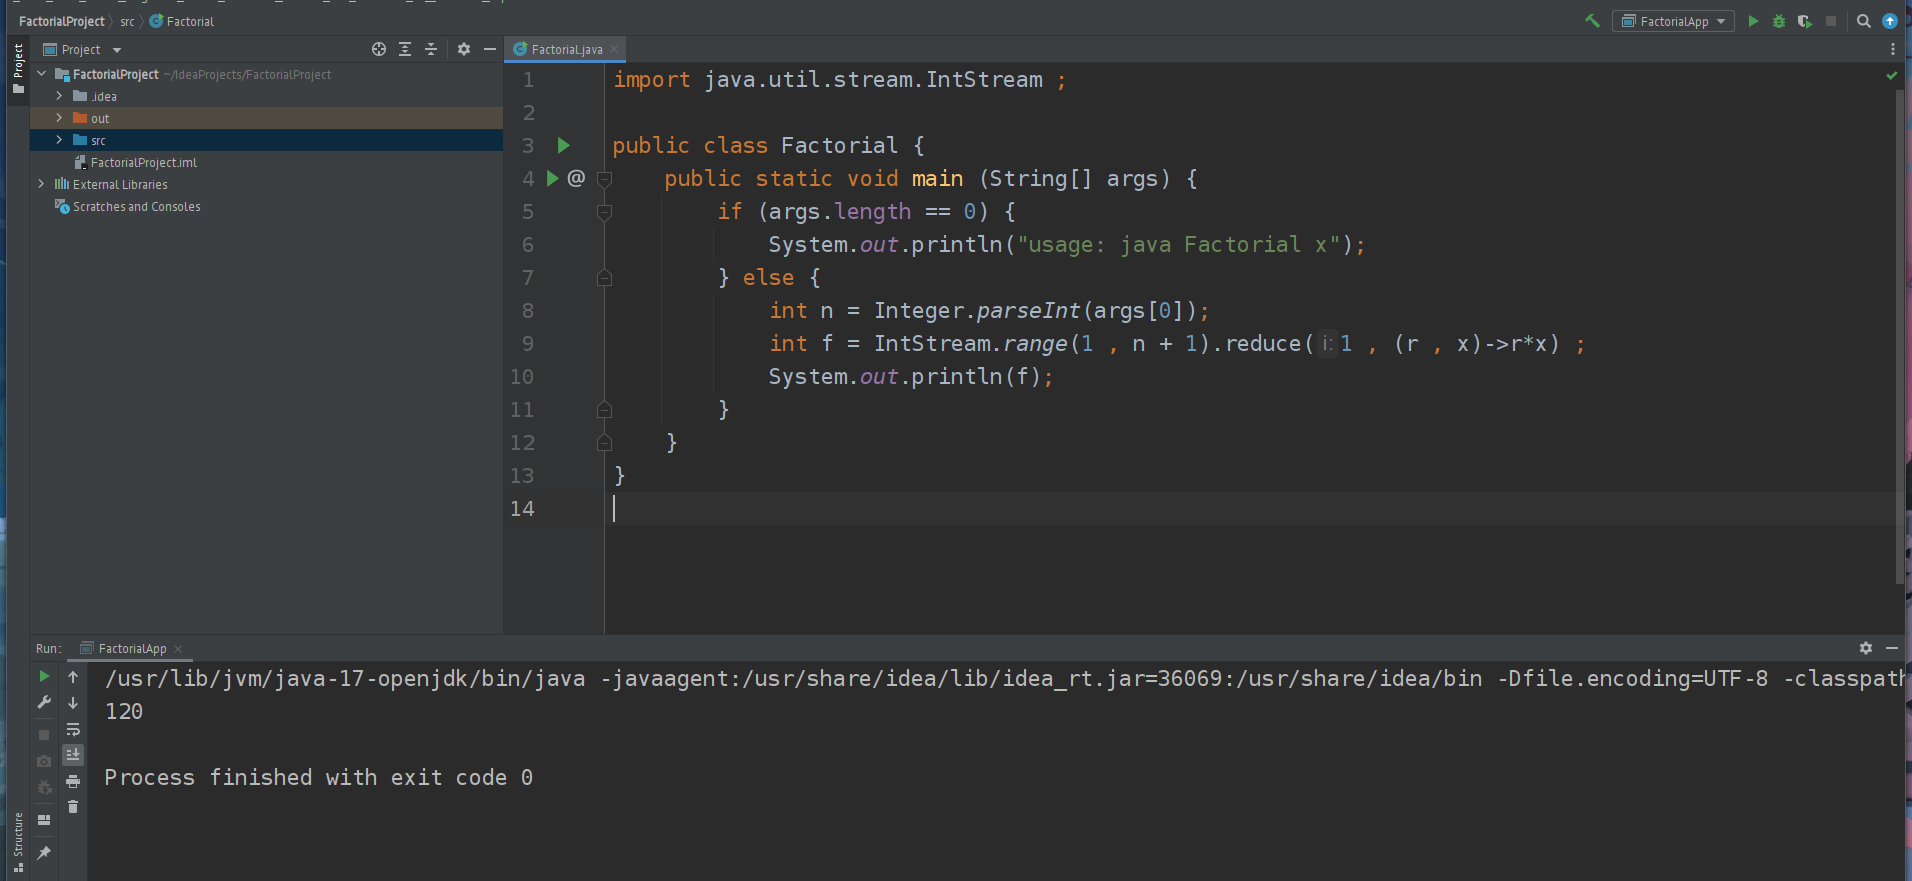
\includegraphics[width=\textwidth]{intelliji}
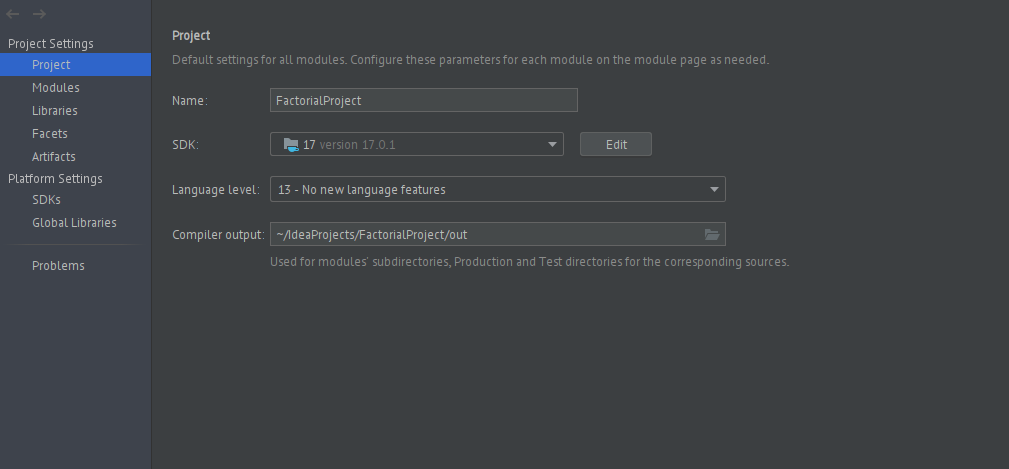
\includegraphics[width=\textwidth]{settings}

\end{document}
